\documentclass[11pt]{scrartcl}

\usepackage{ucs}
\usepackage[utf8x]{inputenc}
\usepackage{ngerman}
\usepackage{amsmath,amssymb,amstext}
\usepackage{graphicx}
\usepackage[automark]{scrpage2}
\usepackage{pgfplots}
\usepackage{chngcntr}
\usepackage[left=3cm, right=3cm, top=3cm, bottom=3cm]{geometry}


\counterwithin{figure}{section}

\pagestyle{scrheadings}

\title{Dykstra}
\author{Finn Jannsen, Philipp Schwarz}
\date{\today{}}

\begin{document}

\maketitle

\tableofcontents

\section{Einführung}
	\label{sec:einfuehrung}
	
	Diese Dokumentation beschreibt die Implementation von Dykstra für einen gewichteten Graphen aus einer Adjazenzmatrix, als auch einer Adjazenzliste.
	In Abschnitt \ref{sec:implementation} wird darauf eingegangen, wie der Algorithmus realisiert wurde.
	Anschließend wird in Abschnitt \ref{sec:veri} geprüft, ob die Implementation korrekt funktioniert 
	und in Abschnitt \ref{sec:aufwand} die Performance auf den beiden Graphen verglichen.

\section{Implementation}
	\label{sec:implementation}
	
	Der Algorithmus wurde als Klasse realisiert, die ein Interface implementiert, welches es ermöglicht, einfach weitere Implementationen, sofern dies gewünscht wird, zu schreiben.
	
	\subsection{Aufbau}
		\label{sec:codeStruc}
		
		Um die Struktur zu verdeutlichen, ist unter \ref{figure:uml} ein UML-Diagramm zu sehen, welches die Verbindungen der einzelnen Klassen und Interfaces beinhält.
		Die Adjazenzmatrix und Adjazenzliste sind hier jeweils GraphMatrix und GraphList. 

\begin{figure}
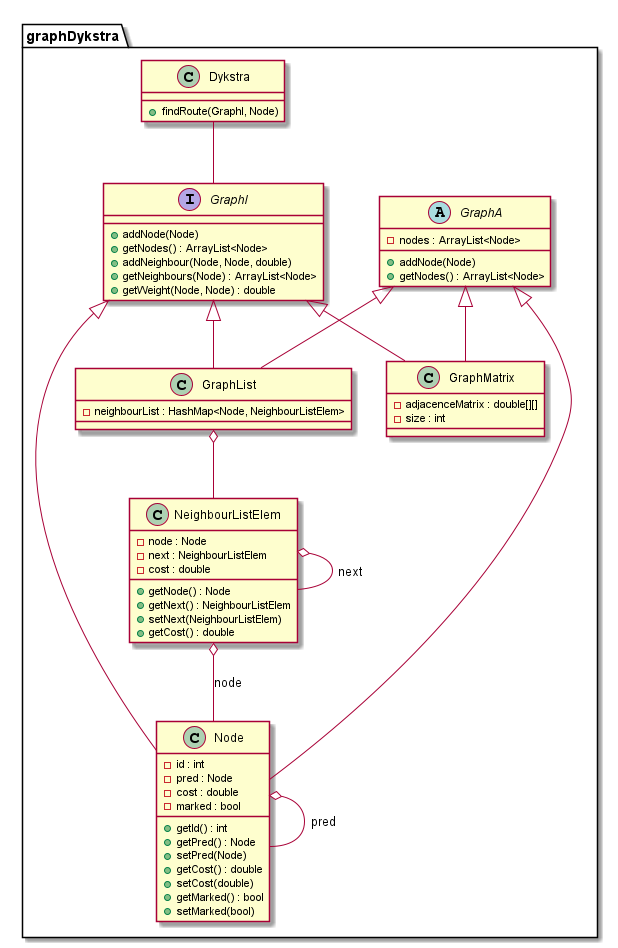
\includegraphics[width=\linewidth]{A9.png}
\caption{UML-Diagramm}
\label{figure:uml}
\end{figure}

		Die Adjazenzmatrix beinhält einen 2-Dimensionalen Array zum Speichern des Graphen, während die Adjazenzliste eine 1-Dimensionale Liste von Nodes ist, welche jeweils auf ihre Kanten verweisen.

	\subsection{Algorithmus}
		\label{sec:algo}

		Der eigentliche Algorithmus zum Berechnen der schnellsten Pfade mit Dijkstra ist unter \ref{figure:dykstra} zu sehen.
		Bei diesem werden zuerst alle Nodes des Graphen initialisiert und anschließend alle Nachbarn des Startknoten in eine PriorityQueue, die nach den Kosten um zu dem Knoten zu kommen, priorisiert ist. Danach wird die PriorityQueue durchgearbeitet, jeder Nachbar des aktuellen Knoten hinzugefügt der noch nicht makiert ist und bei jedem Nachbarn geprüft, ob der Weg über den aktuellen Knoten schneller ist, als bisher bekannt. Wenn dies der Fall ist, wird sich das neue Gewicht und der aktuelle Knoten im Nachbar gemerkt. In jedem Fall wird der aktuelle Knoten als abgearbeitet makiert. Am Ende, wenn die PriorityQueue leer ist, steht sicher, dass der kürzeste Weg vom Endknoten der ist, der herauskommt, wenn den gespeicherten vorherigen Knoten gefolgt wird.

		
\section{Testen und Verifikation}
\label{sec:vertests}

	\subsection{Verifizieren}
		\label{sec:veri}
		
		Der Algorithmus wurde auf seine korrekte Funktionalität getestet.
		Hierzu zählt das Hinzufügen mittels randomisierter Sequenzen, die Anwendung von Dykstra und das Überprüfen des kürzesten Weges.
		Alle Tests wurden erfolgreich mit unterschiedlichen Eingabewerten absolviert.
	
	\subsection{Aufwandsanalyse}
		\label{sec:aufwand}
		
		Für die Aufwandsanalyse wurden die beiden Graphen mit $10^n$ Werten gefüllt, wobei die Werte randomisiert und $n=1,...,4$ war (Der Arbeisspeicher für $10^5$ war ungenügend. Für Durschnittswerte wurden die Tests 30 mal durchgeführt.
		Beobachtet wurden die Rechenoperationen bei der Ausführung von Dykstra. Die Ergebnisse sind unter \ref{figure:quanTest} ersichtlich. Anhand der Anzahl an Operationen lässt sich der Asymptotische Zeitaufwand annähernd wie folgt eingrenzen:
		\begin{equation*}
		T(n) = \mathcal{O}(n*ln(n))
		\end{equation*}

		Auch kann man sehen, dass die Anzahl an Rechenoperationen bei der Adjazenzliste höher ist, als die der Adjazenzmatrix. Dafür braucht die Adjazenzmatrix jedoch aufgrund der Array-Allokierung wesentlich mehr Speicher. Unter anderem wurde festgestellt, dass sich zwischen $10^3$ und $10^4$ Nodes fast nur noch eine 10-er Potenz hinzukommt.


\begin{figure}
    \newcommand{\rsCol}{blue}
    \newcommand{\qsCol}{red}
    \newcommand{\bestAvgMark}{square*}
    \newcommand{\transparent}{0.8}
    \makebox[\textwidth][c]{
    \begin{tikzpicture}
        \begin{loglogaxis}[
                title={\large Berechnung Operationen},
                height=10cm,
                width=17cm,
                grid=major,
                x tick label style={
                /pgf/number format/1000 sep=},
                ylabel=Operationen,
                xlabel=Anzahl Elemente,
                enlargelimits=0.05,
                legend style={at={(0.5,-0.15)},
                anchor=north,legend columns=1},
            ]
            \addplot[color=\rsCol,mark=\bestAvgMark,opacity=\transparent]
                coordinates {(1,0)(10,77)(100,2223)(1000,30313)(10000,314745)};
            \addplot[color=\qsCol,mark=\bestAvgMark,opacity=\transparent]
                coordinates {(1,0)(10,138)(100,2301)(1000,30430)(10000,314828)};
            \legend{Adjazenzmatrix, Adjazenzliste}
        \end{loglogaxis}
    \end{tikzpicture}
    }
    \caption{Quantitativer Vergleich von Adjazenzmatrix und Adjazenzliste}
    \label{figure:quanTest}
\end{figure}

\begin{figure}

\begin{small}
\begin{verbatim}
public static void findRoute(GraphI graph, Node start, Counter counter) {
    Queue<Node> rand = new PriorityQueue<>();

    // 1
    // init every node
    for(Node n : graph.getNodes()) {
        n.setPred(null);
        n.setCost(Double.MAX_VALUE);
        n.setMarked(false);
    }
    // init start node
    start.setPred(start);
    start.setCost(0.0);
    start.setMarked(true);

    // 2
    // fill rand with adjacence nodes of start and init the neighbour nodes of start
    for(Node n : graph.getNeighbours(start)) {
        if (counter != null) {
            counter.increaseCount();
            counter.increaseCount();
        }
        n.setCost(graph.getWeight(start, n));
        n.setPred(start);
        rand.add(n);
    }

    // 3
    // process every node starting with the lowest cost one 
    // (automatically, since this is a prioriry queue, sorted after the cost
    while(!rand.isEmpty()) {
        if (counter != null) {
            counter.increaseCount();
        }
        Node v = rand.poll();
        v.setMarked(true);

        // process every node in rand that is not marked
        for(Node k : graph.getNeighbours(v)) {
            // 3.1
            if (!k.getMarked()) {
                // 3.2
                if (counter != null) {
                    counter.increaseCount();
                    counter.increaseCount();
                }
                double VKCost = v.getCost() + graph.getWeight(v, k);
                if(k.getCost() > VKCost) { 
                    // check if the cost to go to this node via the previous node
                    // is faster than currently known
                    k.setCost(VKCost);
                    k.setPred(v);
                }
                // 3.3
                rand.add(k);
            }
        }
    }
}
\end{verbatim}
\end{small}
\caption{Code-Ausschnitt Dykstra}
\label{figure:dykstra}
\end{figure}

\end{document}